
\section{Regularization}

\begin{frame}{Regularization: Background}
    \only<1-5>{
        \begin{tikzpicture}
            \node[] at (-5.25, -3) {};
            \node[] at (5.25, 3) {};

            \only<1>{
                \node[align=left, text width=10.5cm] at (0, 0) {
                    \textbf{Regularization}: A set of techniques to explicitly reduce the complexity of our models (to reduce overfitting), by encouraging them to learn broader and more general patterns in the training data instead of memorizing it
                };
            }

            \only<2-3>{
                \node[anchor=west] at (-3.8, 2.5) {
                    $y \sim \beta_0 + \beta_1 * x_1 + \beta_2 * x_2$
                };
            }
            \only<4>{
                \node[anchor=west] at (-3.8, 2.5) {
                    $y \sim \beta_0 + \beta_1 * x_1 + \beta_2 * x_2 + \beta_3 * x_3 + \beta_4 * x_4$
                };
            }

            \only<3-4>{
                \node[draw=black, fill=white] at (0, -0.5){
                    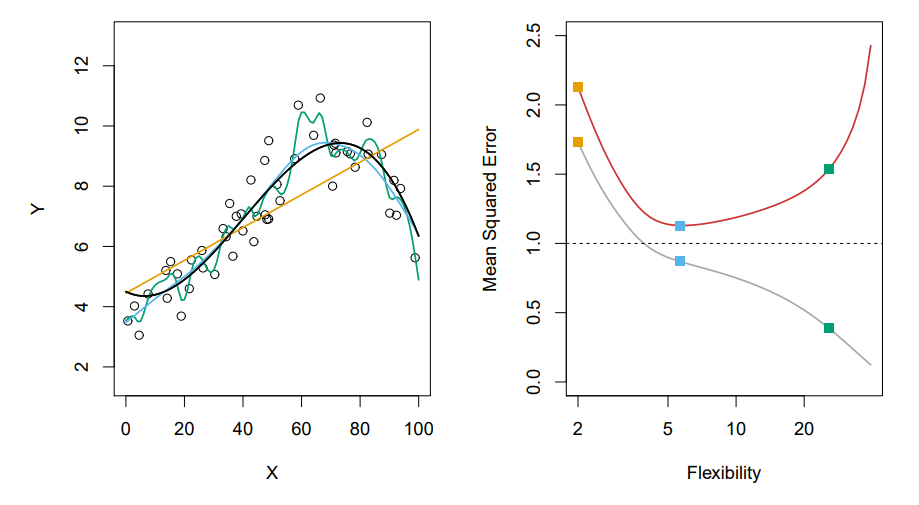
\includegraphics[width=8cm]{data/overfitting.png}
                };
            }

            \only<5>{
                \PythonInputNode{1}{(-4, 2)}{code}{0.9\textwidth}{7}{
                    import pandas as pd^^J
                    ^^J
                    ^^J
                    df = pd.read_csv('/Users/esten/Downloads/Auto.csv')^^J
                    train = df.iloc[:int(len(df) * 0.8)]^^J
                    validation = df.iloc[int(len(df) * 0.8):]^^J
                    ^^J
                    print(f'Using {len(train)} samples for training')^^J
                    print(f'Using {len(validation)} samples for validation')^^J
                }
                \PythonOutputNode{1}{($ (code.south west) + (0.11, -0.2) $)}{output}{0.791\textwidth}{7}{
                    Using 317 samples for training^^J
                    Using 80 samples for validation^^J
                }
            }
        \end{tikzpicture}
    }
    \only<6-7>{
        \begin{enumerate}
            \item Variable selection
            \begin{enumerate}
                \item[a.] Best subset selection
                \item[b.] Forward stepwise selection
                \item[c.] Backward stepwise selection
            \end{enumerate}
            \item Shrinkage
            \begin{enumerate}
                \alert<7>{\item[a.] LASSO}
                \alert<7>{\item[b.] Ridge regression}
            \end{enumerate}
            \item Dimensionality reduction: Lecture 6 and self-study
        \end{enumerate}
    }
\end{frame}

\section{Variable selection}

\newcommand{\autoplot}[1]{
    \nextgroupplot[
        title=\scriptsize{#1},
        every axis title/.style={at={(0.5,1.15)}},
        xmajorticks=false,
        xmajorgrids=true,
        ymajorticks=false,
        ymajorgrids=true
    ]
        \addplot[
            only marks,
            mark=*,
            color=blue,
            opacity=0.25
        ] table[
            col sep=comma,
            y=mpg,
            x=#1
        ] {data/Auto.csv};
}

\newsavebox{\predictors}
\sbox{\predictors}{
    \begin{tikzpicture}
        \begin{groupplot}[
            group style={
                group size=3 by 2,
                horizontal sep=0.5cm
            },
            ticklabel style = {font=\tiny},
            height=3.9cm,
            width=3.9cm
        ]
            \autoplot{cylinders}
            \autoplot{displacement}
            \autoplot{horsepower}
            \autoplot{weight}
            \autoplot{acceleration}
            \autoplot{year}
        \end{groupplot}
    \end{tikzpicture}
}

\begin{frame}{Variable selection: Motivation}
    \begin{tikzpicture}
        \node[] at (-5.25, -3) {};
        \node[] at (5.25, 3) {};

        \only<1-3>{
            \node[align=flush left, anchor=north west, text width=10.5cm] (insight) at (-5.2, 3) {
                The number of predictors we are using in our linear model directly impacts its complexity, allowing us to balance the bias-variance trade off by varying the number of predictors.
            };
        }
        \only<2-3>{
            \node[align=flush left, anchor=north west, text width=10cm] (motivation) at ($ (insight.south west) + (0, 0) $) {
                Fewer predictors also mean that
                \begin{itemize}
                    \alert<3>{\item We avoid problems due to collinearity.}
                    \item There are less coefficients to be interpreted.
                \end{itemize}
            };
        }
        \only<4-5>{
            \node[align=flush left, text width=10.5cm] at (0, 0) {
                \textbf{Formal problem specification}\\
                We have a set of predictors $P=\{x_0, x_1, ...\}$ and a target variable $y$, and we want to find the subset $p \subseteq P$ that yields \alert<5>{the best (linear) model} for predicting $y$.
            };
        }
        \only<6>{
            \node[] at (0, 0) {
                \usebox{\predictors}
            };
        }
    \end{tikzpicture}
\end{frame}

\begin{frame}[t]{Variable selection: Best subset selection}
    \only<1,4>{
        \textbf{Problem}\\
        We have a set of predictors $P=\{x_0, x_1, ...\}$ and a target variable $y$, and we want to find the subset $p \subseteq P$ that yields the best (linear) model for predicting $y$.\\
        \vspace{0.25cm}
        \textbf{Solution}\\
        Train models on all subsets $p$ and select the best one.
    }
    \only<2-3>{
        \begin{tikzpicture}
            \node[] at (-5.25, -3) {};
            \node[] at (5.25, 3) {};

            \PythonInputNode{1}{(-5, 2.5)}{code}{0.95\textwidth}{6}{
import numpy as np^^J
^^J
from itertools import chain, combinations^^J
from sklearn.linear_model import LinearRegression^^J
from sklearn.metrics import mean_squared_error^^J
^^J
subsets = list(chain.from_iterable(combinations(predictors, r) \^^J
{ }{ }{ }{ }{ }{ }{ }{ }{ }{ }{ }{ }{ }{ }{ }for r in range(len(predictors)+1)))^^J
^^J
best = \{'mse': float('inf'), 'subset': None\}^^J
^^J
for subset in subsets:^^J
{ }{ }{ }{ }if len(subset) == 0:^^J
{ }{ }{ }{ }{ }{ }{ }{ }continue^^J
^^J
{ }{ }{ }{ }model = LinearRegression()^^J
{ }{ }{ }{ }model.fit(train[list(subset)], train[target])^^J
{ }{ }{ }{ }predictions = model.predict(validation[list(subset)])^^J
{ }{ }{ }{ }mse = mean_squared_error(validation[target], predictions)^^J
^^J
{ }{ }{ }{ }best = best if mse > best['mse'] else  \{'mse': mse, 'subset': subset\}^^J
^^J
print(f'MSE: \{best["mse"]:.2f\}, predictors: \{best["subset"]\}')^^J
            }
            \PythonOutputNode{1}{($ (code.south west) + (0.11, -0.2) $)}{output}{0.881\textwidth}{6}{
MSE: 29.68, predictors: ('cylinders', 'displacement', 'horsepower', 'weight', 'year')^^J
            }

        \only<3>{
            \node[draw=red, thick, minimum height=0.3cm, minimum width=1.9cm] at (-1.9, -2.55) {};
        }
        \end{tikzpicture}
    }
    \only<4>{

        \textcolor{green}{+} \textbf{Positives}\\
        \textbullet{ }Guaranteed to find the optimal solution.\\
        \textbullet{ }Simple implementation\\

        \textcolor{red}{-} \textbf{Drawbacks}\\
        \textbullet{ }Need to train many ($2^{|P|}$) models.
    }
    \only<5>{
        \centering
        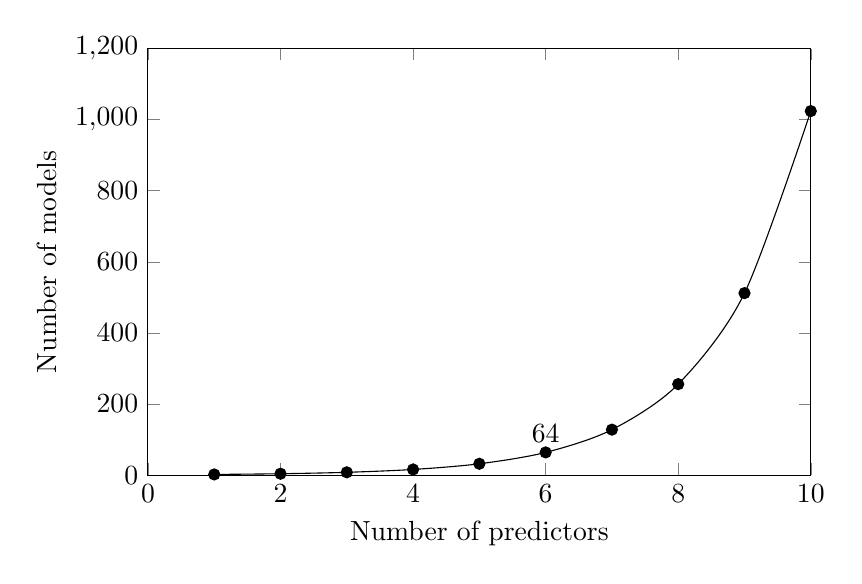
\begin{tikzpicture}
            \begin{axis}[
                smooth,
                xmin=0,
                xmax=10,
                ymin=0,
                ymax=1200,
                xlabel={Number of predictors},
                ylabel={Number of models},
                height=7cm,
                width=10cm
            ]
                \addplot[mark=*] coordinates {
                    (1, 2^1)
                    (2, 2^2)
                    (3, 2^3)
                    (4, 2^4)
                    (5, 2^5)
                    (6, 2^6)
                    (7, 2^7)
                    (8, 2^8)
                    (9, 2^9)
                    (10, 2^10)
                };
                \node[anchor=south] at (axis cs: 6, 2^6) {64};
            \end{axis}
        \end{tikzpicture}
    }
\end{frame}

 \begin{frame}[t]{Variable selection: Forward stepwise selection}
    \only<1-2,13>{
        \textbf{Problem}\\
        We have a set of predictors $P=\{x_0, x_1, ...\}$ and a target variable $y$, and we want to find the subset $p \subseteq P$ that yields the best (linear) model for predicting $y$.\\
        \vspace{0.25cm}
        \textbf{Solution}\\
        Start by fitting a model with no predictors. Iteratively add the predictor that yields the \alert<2>{best model} until all are included.\\

        \only<13>{
            \vspace{0.25cm}
            \textcolor{green}{+}{ }\textbf{Positives}\\
            \textbullet{ }Need to train fewer models.\\
            \vspace{0.25cm}
            \textcolor{red}{-}{ }\textbf{Drawbacks}\\
            \textbullet{ }Not guaranteed to find the optimal solution.\\
        }
    }

    \only<3-10>{
        \def\nodefont{\fontsize{4}{4}\linespread{0.85}\selectfont}
        \def\hsep{1.6}
        \def\vsep{0.75}
        \begin{tikzpicture}
            \node[draw=black, align=center, font=\nodefont] (n00) at (0, 0 * \vsep) {
                $y \sim \mathbbm{1}$\\
                $mse=146.47$
            };

            \node[] at (6.5 * \hsep, 3.3 * \vsep) {};
            \node[] at (-0.32 * \hsep, -3.3 * \vsep) {};

            \only<4>{
                \node[draw=black, align=center, font=\nodefont, color=black] (n11) at (\hsep, 2.5 * \vsep) {
                    $y \sim cylinders$\\
                    $67.96$
                };
                \node[draw=black, align=center, font=\nodefont, color=black] (n12) at (\hsep, 1.5 * \vsep) {
                    $y \sim year$\\
                    $61.56$
                };
                \node[draw=black, align=center, font=\nodefont, color=black] (n13) at (\hsep, 0.5 * \vsep) {
                    $y \sim acceleration$\\
                    $119.72$
                };
                \node[draw=black, align=center, font=\nodefont] (n14) at (\hsep, -0.5 * \vsep) {
                    $y \sim weight$\\
                    $61.18$
                };
                \node[draw=black, align=center, font=\nodefont, color=black] (n15) at (\hsep, -1.5 * \vsep) {
                    $y \sim horsepower$\\
                    $65.75$
                };
                \node[draw=black, align=center, font=\nodefont, color=black] (n16) at (\hsep, -2.5 * \vsep) {
                    $y \sim displacement$\\
                    $63.84$
                };


                \draw[black] (n00.east) -- (n11.west);
                \draw[black] (n00.east) -- (n12.west);
                \draw[black] (n00.east) -- (n13.west);
                \draw[black] (n00.east) -- (n14.west);
                \draw[black] (n00.east) -- (n15.west);
                \draw[black] (n00.east) -- (n16.west);
            }
            \only<5-10>{
                \node[draw=gray!25, align=center, font=\nodefont, color=gray!25] (n11) at (\hsep, 2.5 * \vsep) {
                    $y \sim cylinders$\\
                    $67.96$
                };
                \node[draw=gray!25, align=center, font=\nodefont, color=gray!25] (n12) at (\hsep, 1.5 * \vsep) {
                    $y \sim year$\\
                    $61.56$
                };
                \node[draw=gray!25, align=center, font=\nodefont, color=gray!25] (n13) at (\hsep, 0.5 * \vsep) {
                    $y \sim acceleration$\\
                    $119.72$
                };
                \node[draw=black, align=center, font=\nodefont] (n14) at (\hsep, -0.5 * \vsep) {
                    $y \sim weight$\\
                    $61.18$
                };
                \node[draw=gray!25, align=center, font=\nodefont, color=gray!25] (n15) at (\hsep, -1.5 * \vsep) {
                    $y \sim horsepower$\\
                    $65.75$
                };
                \node[draw=gray!25, align=center, font=\nodefont, color=gray!25] (n16) at (\hsep, -2.5 * \vsep) {
                    $y \sim displacement$\\
                    $63.84$
                };


                \draw[gray!25] (n00.east) -- (n11.west);
                \draw[gray!25] (n00.east) -- (n12.west);
                \draw[gray!25] (n00.east) -- (n13.west);
                \draw[black] (n00.east) -- (n14.west);
                \draw[gray!25] (n00.east) -- (n15.west);
                \draw[gray!25] (n00.east) -- (n16.west);
            }
            \only<6>{
                \node[draw=black, align=center, font=\nodefont, color=black] (n21) at (2 * \hsep, 2.5 * \vsep) {
                    $\begin{aligned}
                        y\sim&weight +\\[-0.8em]
                        &cylinders
                    \end{aligned}$\\
                    $60.02$
                };
                \node[draw=black, align=center, font=\nodefont] (n22) at (2 * \hsep, 1.25 * \vsep) {
                    $\begin{aligned}
                        y\sim&weight +\\[-0.8em]
                        &year
                    \end{aligned}$\\
                    $29.84$
                };
                \node[draw=black, align=center, font=\nodefont, color=black] (n23) at (2 * \hsep, 0 * \vsep) {
                    $\begin{aligned}
                        y\sim&weight +\\[-0.8em]
                        &acceleration
                    \end{aligned}$\\
                    $60.01$
                };
                \node[draw=black, align=center, font=\nodefont, color=black] (n24) at (2 * \hsep, -1.25 * \vsep) {
                    $\begin{aligned}
                        y\sim&weight +\\[-0.8em]
                        &horsepower
                    \end{aligned}$\\
                    $58.59$
                };
                \node[draw=black, align=center, font=\nodefont, color=black] (n25) at (2 * \hsep, -2.5 * \vsep) {
                    $\begin{aligned}
                        y\sim&weight +\\[-0.8em]
                        &displacement
                    \end{aligned}$\\
                    $59.91$
                };

                \draw[black] (n14.east) -- (n21.west);
                \draw[black] (n14.east) -- (n22.west);
                \draw[black] (n14.east) -- (n23.west);
                \draw[black] (n14.east) -- (n24.west);
                \draw[black] (n14.east) -- (n25.west);
            }
            \only<7-10>{
                \node[draw=gray!25, align=center, font=\nodefont, color=gray!25] (n21) at (2 * \hsep, 2.5 * \vsep) {
                    $\begin{aligned}
                        y\sim&weight +\\[-0.8em]
                        &cylinders
                    \end{aligned}$\\
                    $60.02$
                };
                \node[draw=black, align=center, font=\nodefont] (n22) at (2 * \hsep, 1.25 * \vsep) {
                    $\begin{aligned}
                        y\sim&weight +\\[-0.8em]
                        &year
                    \end{aligned}$\\
                    $29.84$
                };
                \node[draw=gray!25, align=center, font=\nodefont, color=gray!25] (n23) at (2 * \hsep, 0 * \vsep) {
                    $\begin{aligned}
                        y\sim&weight +\\[-0.8em]
                        &acceleration
                    \end{aligned}$\\
                    $60.01$
                };
                \node[draw=gray!25, align=center, font=\nodefont, color=gray!25] (n24) at (2 * \hsep, -1.25 * \vsep) {
                    $\begin{aligned}
                        y\sim&weight +\\[-0.8em]
                        &horsepower
                    \end{aligned}$\\
                    $58.59$
                };
                \node[draw=gray!25, align=center, font=\nodefont, color=gray!25] (n25) at (2 * \hsep, -2.5 * \vsep) {
                    $\begin{aligned}
                        y\sim&weight +\\[-0.8em]
                        &displacement
                    \end{aligned}$\\
                    $59.91$
                };

                \draw[gray!25] (n14.east) -- (n21.west);
                \draw[black] (n14.east) -- (n22.west);
                \draw[gray!25] (n14.east) -- (n23.west);
                \draw[gray!25] (n14.east) -- (n24.west);
                \draw[gray!25] (n14.east) -- (n25.west);
            }
            \only<7>{
                \node[draw=black, align=center, font=\nodefont, color=black] (n31) at (3 * \hsep, 2.25 * \vsep) {
                    $\begin{aligned}
                        y\sim&weight +\\[-0.8em]
                        &year +\\[-0.8em]
                        &cylinders
                    \end{aligned}$\\
                    $29.91$
                };
                \node[draw=black, align=center, font=\nodefont, color=black] (n32) at (3 * \hsep, 0.75 * \vsep) {
                    $\begin{aligned}
                        y\sim&weight +\\[-0.8em]
                        &year +\\[-0.8em]
                        &acceleration
                    \end{aligned}$\\
                    $29.99$
                };
                \node[draw=black, align=center, font=\nodefont] (n33) at (3 * \hsep, -0.75 * \vsep) {
                    $\begin{aligned}
                        y\sim&weight +\\[-0.8em]
                        &year +\\[-0.8em]
                        &horsepower
                    \end{aligned}$\\
                    $29.85$
                };
                \node[draw=black, align=center, font=\nodefont, color=black] (n34) at (3 * \hsep, -2.25 * \vsep) {
                    $\begin{aligned}
                        y\sim&weight +\\[-0.8em]
                        &year +\\[-0.8em]
                        &displacement
                    \end{aligned}$\\
                    $29.96$
                };

                \draw[black] (n22.east) -- (n31.west);
                \draw[black] (n22.east) -- (n32.west);
                \draw[black] (n22.east) -- (n33.west);
                \draw[black] (n22.east) -- (n34.west);
            }
            \only<8-10>{
                \node[draw=gray!25, align=center, font=\nodefont, color=gray!25] (n31) at (3 * \hsep, 2.25 * \vsep) {
                    $\begin{aligned}
                        y\sim&weight +\\[-0.8em]
                        &year +\\[-0.8em]
                        &cylinders
                    \end{aligned}$\\
                    $29.91$
                };
                \node[draw=gray!25, align=center, font=\nodefont, color=gray!25] (n32) at (3 * \hsep, 0.75 * \vsep) {
                    $\begin{aligned}
                        y\sim&weight +\\[-0.8em]
                        &year +\\[-0.8em]
                        &acceleration
                    \end{aligned}$\\
                    $29.99$
                };
                \node[draw=black, align=center, font=\nodefont] (n33) at (3 * \hsep, -0.75 * \vsep) {
                    $\begin{aligned}
                        y\sim&weight +\\[-0.8em]
                        &year +\\[-0.8em]
                        &horsepower
                    \end{aligned}$\\
                    $29.85$
                };
                \node[draw=gray!25, align=center, font=\nodefont, color=gray!25] (n34) at (3 * \hsep, -2.25 * \vsep) {
                    $\begin{aligned}
                        y\sim&weight +\\[-0.8em]
                        &year +\\[-0.8em]
                        &displacement
                    \end{aligned}$\\
                    $29.96$
                };

                \draw[gray!25] (n22.east) -- (n31.west);
                \draw[gray!25] (n22.east) -- (n32.west);
                \draw[black] (n22.east) -- (n33.west);
                \draw[gray!25] (n22.east) -- (n34.west);
            }
            \only<8>{
                \node[draw=black, align=center, font=\nodefont, color=black] (n41) at (4 * \hsep, 1.75 * \vsep) {
                    $\begin{aligned}
                        y\sim&weight +\\[-0.8em]
                        &year +\\[-0.8em]
                        &horsepower +\\[-0.8em]
                        &cylinders
                    \end{aligned}$\\
                    $29.87$
                };
                \node[draw=black, align=center, font=\nodefont, color=black] (n42) at (4 * \hsep, 0 * \vsep) {
                    $\begin{aligned}
                        y\sim&weight +\\[-0.8em]
                        &year +\\[-0.8em]
                        &horsepower +\\[-0.8em]
                        &acceleration
                    \end{aligned}$\\
                    $30.29$
                };
                \node[draw=black, align=center, font=\nodefont, color=black] (n43) at (4 * \hsep, -1.75 * \vsep) {
                    $\begin{aligned}
                        y\sim&weight +\\[-0.8em]
                        &year +\\[-0.8em]
                        &horsepower +\\[-0.8em]
                        &displacement
                    \end{aligned}$\\
                    $29.95$
                };

                \draw[black] (n33.east) -- (n41.west);
                \draw[black] (n33.east) -- (n42.west);
                \draw[black] (n33.east) -- (n43.west);
            }
            \only<9-10>{
                \node[draw=black, align=center, font=\nodefont, color=black] (n41) at (4 * \hsep, 1.75 * \vsep) {
                    $\begin{aligned}
                        y\sim&weight +\\[-0.8em]
                        &year +\\[-0.8em]
                        &horsepower +\\[-0.8em]
                        &cylinders
                    \end{aligned}$\\
                    $29.87$
                };
                \node[draw=gray!25, align=center, font=\nodefont, color=gray!25] (n42) at (4 * \hsep, 0 * \vsep) {
                    $\begin{aligned}
                        y\sim&weight +\\[-0.8em]
                        &year +\\[-0.8em]
                        &horsepower +\\[-0.8em]
                        &acceleration
                    \end{aligned}$\\
                    $30.29$
                };
                \node[draw=gray!25, align=center, font=\nodefont, color=gray!25] (n43) at (4 * \hsep, -1.75 * \vsep) {
                    $\begin{aligned}
                        y\sim&weight +\\[-0.8em]
                        &year +\\[-0.8em]
                        &horsepower +\\[-0.8em]
                        &displacement
                    \end{aligned}$\\
                    $29.95$
                };

                \draw[black] (n33.east) -- (n41.west);
                \draw[gray!25] (n33.east) -- (n42.west);
                \draw[gray!25] (n33.east) -- (n43.west);
            }
            \only<9>{
                \node[draw=black, align=center, font=\nodefont] (n51) at (5 * \hsep, 1 * \vsep) {
                    $\begin{aligned}
                        y\sim&weight +\\[-0.8em]
                        &year +\\[-0.8em]
                        &horsepower +\\[-0.8em]
                        &cylinders +\\[-0.8em]
                        &acceleration
                    \end{aligned}$\\
                    $29.68$
                };
                \node[draw=black, align=center, font=\nodefont, color=black] (n52) at (5 * \hsep, -1 * \vsep) {
                    $\begin{aligned}
                        y\sim&weight +\\[-0.8em]
                        &year +\\[-0.8em]
                        &horsepower +\\[-0.8em]
                        &cylinders +\\[-0.8em]
                        &displacement
                    \end{aligned}$\\
                    $30.47$
                };

                \draw[black] (n41.east) -- (n51.west);
                \draw[black] (n41.east) -- (n52.west);
            }
            \only<10>{
                \node[draw=black, align=center, font=\nodefont] (n51) at (5 * \hsep, 1 * \vsep) {
                    $\begin{aligned}
                        y\sim&weight +\\[-0.8em]
                        &year +\\[-0.8em]
                        &horsepower +\\[-0.8em]
                        &cylinders +\\[-0.8em]
                        &acceleration
                    \end{aligned}$\\
                    $29.68$
                };
                \node[draw=gray!25, align=center, font=\nodefont, color=gray!25] (n52) at (5 * \hsep, -1 * \vsep) {
                    $\begin{aligned}
                        y\sim&weight +\\[-0.8em]
                        &year +\\[-0.8em]
                        &horsepower +\\[-0.8em]
                        &cylinders +\\[-0.8em]
                        &displacement
                    \end{aligned}$\\
                    $30.47$
                };

                \draw[black] (n41.east) -- (n51.west);
                \draw[gray!25] (n41.east) -- (n52.west);

                \node[draw=black, align=center, font=\nodefont] (n61) at (6 * \hsep, 0 * \vsep) {
                    $\begin{aligned}
                        y\sim&weight +\\[-0.8em]
                        &year +\\[-0.8em]
                        &horsepower +\\[-0.8em]
                        &cylinders +\\[-0.8em]
                        &acceleration +\\[-0.8em]
                        &displacement
                    \end{aligned}$\\
                    $30.29$
                };

                \draw[black] (n51.east) -- (n61.west);
            }
        \end{tikzpicture}
    }
    \only<11>{
        \centering
        \vspace{0.7cm}
        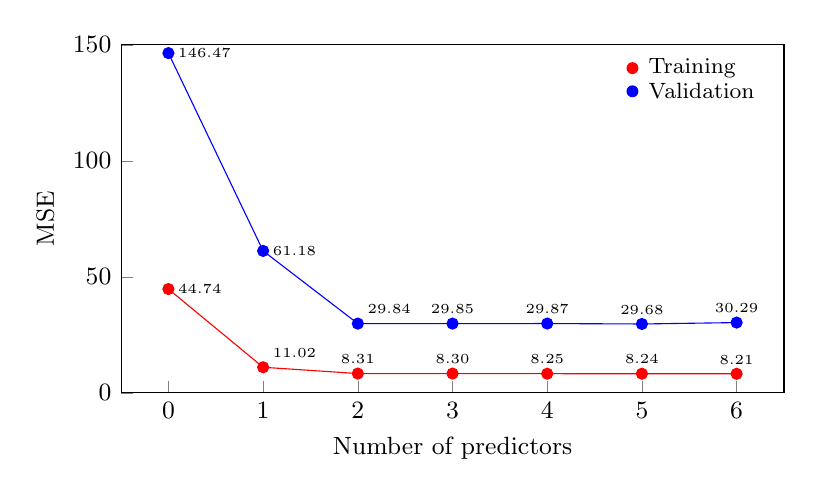
\begin{tikzpicture}
            \begin{axis}[
                xmin=-0.5,
                xmax=6.5,
                ymin=0,
                ymax=150,
                height=6cm,
                width=10cm,
                ytick pos=left,
                xtick pos=bottom,
                ylabel=\small{MSE},
                xlabel=\small{Number of predictors},
                ticklabel style={font=\small},
            ]
                \addplot[red,mark=*] coordinates {
                    (0, 44.74)
                    (1, 11.02)
                    (2, 8.31)
                    (3, 8.31)
                    (4, 8.25)
                    (5, 8.24)
                    (6, 8.21)
                };
                \addplot[blue,mark=*] coordinates {
                    (0, 146.47)
                    (1, 61.18)
                    (2, 29.84)
                    (3, 29.85)
                    (4, 29.87)
                    (5, 29.68)
                    (6, 30.29)
                };

                \node[
                    circle,
                    fill=red,
                    minimum size=4.3pt,
                    inner sep=0pt,
                    label=right:\footnotesize{Training}
                ] at (axis cs: 4.9, 140) {};
                \node[
                    circle,
                    fill=blue,
                    minimum size=4.3pt,
                    inner sep=0pt,
                    label=right:\footnotesize{Validation}
                ] at (axis cs: 4.9, 130) {};

                \node[anchor=west,font=\tiny] at (axis cs: 0, 44.74) {44.74};
                \node[anchor=south west,font=\tiny] at (axis cs: 1, 11.02) {11.02};
                \node[anchor=south,font=\tiny] at (axis cs: 2, 8.31) {8.31};
                \node[anchor=south,font=\tiny] at (axis cs: 3, 8.31) {8.30};
                \node[anchor=south,font=\tiny] at (axis cs: 4, 8.25) {8.25};
                \node[anchor=south,font=\tiny] at (axis cs: 5, 8.24) {8.24};
                \node[anchor=south,font=\tiny] at (axis cs: 6, 8.21) {8.21};

                \node[anchor=west,font=\tiny] at (axis cs: 0, 146.47) {146.47};
                \node[anchor=west,font=\tiny] at (axis cs: 1, 61.18) {61.18};
                \node[anchor=south west,font=\tiny] at (axis cs: 2, 29.84) {29.84};
                \node[anchor=south,font=\tiny] at (axis cs: 3, 29.85) {29.85};
                \node[anchor=south,font=\tiny] at (axis cs: 4, 29.87) {29.87};
                \node[anchor=south,font=\tiny] at (axis cs: 5, 29.68) {29.68};
                \node[anchor=south,font=\tiny] at (axis cs: 6, 30.29) {30.29};

            \end{axis}
        \end{tikzpicture}
    }
    \only<12>{
        \begin{tikzpicture}
            \node[] at (-5.25, -3) {};
            \node[] at (5.25, 3) {};

            \PythonInputNode{1}{(-5, 2.5)}{code}{0.95\textwidth}{4}{
def fit_and_evaluate(train: pd.DataFrame, validation: pd.DataFrame,^^J
{ }{ }{ }{ }{ }{ }{ }{ }{ }{ }{ }{ }{ }{ }{ }{ }{ }{ }{ }{ }{ }predictors: List[str], target: str):^^J
{ }{ }{ }{ }model = LinearRegression()^^J
{ }{ }{ }{ }model.fit(train[predictors], train[target])^^J
^^J
{ }{ }{ }{ }train_predictions = model.predict(train[predictors])^^J
{ }{ }{ }{ }validation_predictions = model.predict(validation[predictors])^^J
^^J
{ }{ }{ }{ }return np.mean((train_predictions - train[target]) ** 2), \^^J
{ }{ }{ }{ }{ }{ }{ }{ }{ }{ }{ }np.mean((validation_predictions - validation[target]) ** 2)^^J
^^J
^^J
predictors = ['cylinders', 'displacement', 'horsepower', 'weight', 'acceleration', 'year']^^J
target = 'mpg'^^J
^^J
train['intercept'] = 1^^J
validation['intercept'] = 1^^J
train_mse, validation_mse = fit_and_evaluate(train, validation, predictors=['intercept'], target=target)^^J
print(f'[]: \{validation_mse:.2f\} (\{train_mse:.2f\})')^^J
^^J
chosen_predictors = []^^J
^^J
while len(chosen_predictors) < len(predictors):^^J
{ }{ }{ }{ }best_predictor = \{'train_mse': None, 'validation_mse': float('inf'),^^J
{ }{ }{ }{ }{ }{ }{ }{ }{ }{ }{ }{ }{ }{ }{ }{ }{ }{ }{ }{ }{ }{ }'predictor': None\}^^J
      ^^J
{ }{ }{ }{ }for predictor in set(predictors) - set(chosen_predictors):^^J
{ }{ }{ }{ }{ }{ }{ }{ }train_mse, validation_mse = fit_and_evaluate(train, validation, predictors=chosen_predictors + [predictor], target=target)^^J
^^J
{ }{ }{ }{ }{ }{ }{ }{ }if validation_mse < best_predictor['validation_mse']:^^J
{ }{ }{ }{ }{ }{ }{ }{ }{ }{ }{ }{ }best_predictor = \{'train_mse': train_mse, 'validation_mse': validation_mse, 'predictor': predictor\}^^J
^^J
{ }{ }{ }{ }chosen_predictors.append(best_predictor['predictor'])^^J
^^J
{ }{ }{ }{ }print(f'\{chosen_predictors\}: \{best_predictor["validation_mse"]:.2f\} (\{best_predictor["train_mse"]:.2f\})')^^J
            }
        \end{tikzpicture}
    }
\end{frame}

\begin{frame}[t]{Variable selection: Backward stepwise selection}
    \only<1-2>{
        \textbf{Problem}\\
        We have a set of predictors $P=\{x_0, x_1, ...\}$ and a target variable $y$, and we want to find the subset $p \subseteq P$ that yields the best (linear) model for predicting $y$.\\
        \vspace{0.25cm}
        \textbf{Solution}\\
        Start by fitting a model with \alert<2>{all} predictors. Iteratively \alert<2>{remove} the predictor that yields the best model until all you have none left.\\
        \vspace{0.25cm}
        \textcolor{green}{+} \textbf{Positives}\\
        \textbullet{ }Need to train fewer models.\\
        \vspace{0.25cm}
        \textcolor{red}{-} \textbf{Drawbacks}\\
        \textbullet{ }Not guaranteed to find the optimal solution.\\
    }
    \only<3>{
        \vspace{3cm}
        \centering
        Does forward and backward stepwise selection yield the same set of predictors?
    }
\end{frame}

\section{Shrinkage}

\def\codewidth{5.2cm}

\begin{frame}{Shrinkage: Outline}
    \definecolor{mse}{HTML}{cc79a7}
    \definecolor{variance}{HTML}{10a47b}
    \begin{tikzpicture}
        \node[] at (-5.25, 3.5) {};
        \node[] at (5.25, -3.5) {};

        \only<1-5, 7-11>{
            \node[] at (0, 3) {
                $y \sim \beta_0 + \alert<2-9>{\beta_1}x_1 + \alert<2-9>{\beta_2}x_2 + \alert<2-9>{\beta_3}x_3 + \alert<2-9>{\beta_4}x_4 + \alert<2-9>{\beta_5}x_5 + \alert<2-9>{\beta_6}x_6$
            };
        }
        \only<3-5, 7-11>{
            \node[] at (0, 2.25) {
                \alert<3>{$\beta_n \rightarrow 0$}
            };
        }
        \only<4-5, 7-11>{
            \node[anchor=north west, align=flush left, text width=10.5cm] at (-5.25, 2) {
                \begin{enumerate}
                    \item $\beta_1 = 0 \implies \text{One less degree of freedom in our function space}$\\
                    \item<7-> $\text{A little more bias} \implies \text{A lot less variance}$\\
                    \item<11> $\text{Parameters depend on eachother} \implies \text{Fewer degrees of freedom}$
                \end{enumerate}
            };
        }
        \only<5>{
            \node[] at (0, -3) {
                $RSS$$ = $$bias^2$$ + $$variance$$ + irreducible\ error$
            };
        }
        \only<6>{
            \node[] at (0, -3) {
                \textcolor{mse}{$RSS$}$ = $$bias^2$$ + $\textcolor{variance}{$variance$}\textcolor{gray!25}{$ + irreducible\ error$}
            };
            \node[inner sep=0pt, draw=black] at (0, 0.5) {
                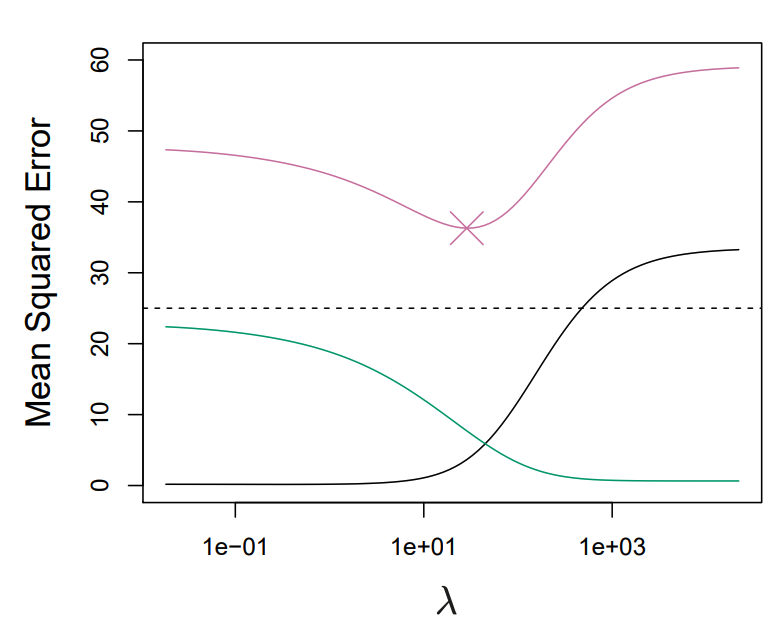
\includegraphics[width=7cm]{data/bias_variance_decomp.png}
            };
        }

        \only<8-10>{
            \node[align=center] (formula) at (0, -1.3) {
                $y \sim \beta_0 + \alert<10>{\beta_1}x_1 + \alert<10>{\beta_2}x_2 + \beta_3x_3 + \beta_4x_4 + \beta_5x_5 + \beta_6x_6$\\
                subject to the constraint\\
                $\sum\limits_{j=1}^p |\beta_j| \leq 1$
            };
        }
        \only<9-10>{
            \node[] at (0, -3) {
                $\beta_1=1, \beta_2=0, \beta_3=0, \ldots$
            };
        }
    \end{tikzpicture}
\end{frame}

\newcommand{\ridgeintuition}[1]{
    \begin{tikzpicture}
        \begin{axis}[
            xmin=-2,
            xmax=5,
            ymin=-2,
            ymax=5,
            axis lines=middle,
            height=7cm,
            width=7cm,
            xtick={-2, -1, 0, 1, 2, 3, 4},
            ytick={-2, -1, 0, 1, 2, 3, 4},
            ticklabel style={font=\footnotesize},
        ]
            \node[] at (axis cs: -0.8, 2.5) {
                \footnotesize{$\beta_2$}
            };
            \node[] at (axis cs: 2.6, -0.8) {
                \footnotesize{$\beta_1$}
            };

            \ifnum#1<9
                \ifnum#1=2
                    \node[cross out, draw=black, thick, inner sep=0pt, minimum size=3pt, orange] at (axis cs: 1, 0) {};
                \fi
                \ifnum#1=3
                    \node[cross out, draw=black, thick, inner sep=0pt, minimum size=3pt, orange] at (axis cs: 1.5, 1.5) {};
                \fi
                \ifnum#1>3
                    \node[cross out, draw=black, thick, inner sep=0pt, minimum size=3pt, orange] at (axis cs: 2.82, 2.7) {};
                \fi
                \ifnum#1=5
                    \node[circle, inner sep=1pt, draw=orange, fill=orange] at (axis cs: 2.14, 1.85) {};
                    \node[anchor=north, text=orange, font=\tiny, inner sep=2.5pt] at (axis cs: 2.14, 1.85) {1};
                \fi
                \ifnum#1=6
                    \node[anchor=north, text=orange, font=\tiny, inner sep=2.5pt] at (axis cs: 2.14, 1.85) {1};
                \fi
                \ifnum#1>5
                    \draw[rotate around={30:(axis cs: 2.82, 2.7)}, orange] (axis cs: 2.82, 2.7) ellipse (1cm and 0.5cm);
                \fi
                \ifnum#1>6
                    \draw[rotate around={30:(axis cs: 2.82, 2.7)}, orange] (axis cs: 2.82, 2.7) ellipse (1.414*1cm and 1.414*0.5cm);
                \fi
                \ifnum#1>7
                    \draw[rotate around={30:(axis cs: 2.82, 2.7)}, orange] (axis cs: 2.82, 2.7) ellipse (1.732*1cm and 1.732*0.5cm);
                \fi
            \fi

            \ifnum#1>8
                \node[cross out, draw=black, thick, inner sep=0pt, minimum size=3pt] at (axis cs: 2.82, 2.7) {};
                \draw[rotate around={30:(axis cs: 2.82, 2.7)}] (axis cs: 2.82, 2.7) ellipse (1cm and 0.5cm);
                \draw[rotate around={30:(axis cs: 2.82, 2.7)}] (axis cs: 2.82, 2.7) ellipse (1.414*1cm and 1.414*0.5cm);
                \draw[rotate around={30:(axis cs: 2.82, 2.7)}] (axis cs: 2.82, 2.7) ellipse (1.732*1cm and 1.732*0.5cm);
            \fi
            \ifnum#1<13
                \ifnum#1>9
                    \node[cross out, draw=black, thick, inner sep=0pt, minimum size=3pt, orange] at (axis cs: 0, 0) {};
                \fi
                \ifnum#1>10
                    \draw[orange] (axis cs: 0, 0) circle (0.78cm);
                \fi
                \ifnum#1>11
                    \draw[orange] (axis cs: 0, 0) circle (1.414*0.78cm);
                    \draw[orange] (axis cs: 0, 0) circle (1.732*0.78cm);
                \fi
            \fi

            \ifnum#1>12
                \node[cross out, draw=black, thick, inner sep=0pt, minimum size=3pt] at (axis cs: 0, 0) {};
                \draw[] (axis cs: 0, 0) circle (0.78cm);
                \draw[] (axis cs: 0, 0) circle (1.414*0.78cm);
                \draw[] (axis cs: 0, 0) circle (1.732*0.78cm);

                \ifnum#1>13
                    \node[cross out, draw=black, thick, inner sep=0pt, minimum size=3pt, orange] at (axis cs: 1.07, 1.4) {};
                \fi
            \fi

        \end{axis}
    \end{tikzpicture}
}

\newcommand{\mseintuitionunivariate}{
    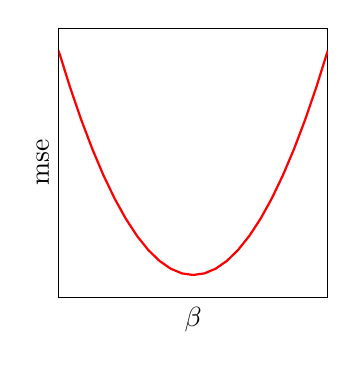
\begin{tikzpicture}
        \begin{axis}[
            height=5cm,
            width=5cm,
            xlabel=$\beta$,
            ylabel=mse,
            ymajorticks=false,
            xmajorticks=false,
            xmin=-1,
            xmax=1
        ]
            \addplot[
                thick,
                red,
                domain=-1:1
            ] {x^2};

        \end{axis}
    \end{tikzpicture}
}

\newcommand{\mseintuitionbivariate}[1]{
    \begin{tikzpicture}
        \begin{axis}[
            height=5cm,
            width=5cm,
            xlabel={$\beta_1$},
            ylabel={$\beta_2$},
            zlabel=mse,
            domain=-3:3,
            y domain=-3:3,
            view={30}{15},
            colormap/viridis,
            grid=major,
            xmajorticks=false,
            ymajorticks=false,
            zmajorticks=false,
            zmin=-0.2
        ]
        \addplot3[surf, samples=30, opacity=0.5] {x^2 + y^2};

        \ifnum#1>0
            \addplot3[
                only marks,
                orange,
                thick,
                mark size=3pt,
                mark=x
            ] coordinates {
                (0, 0, -0.1)
            };
        \fi

        \ifnum#1=2
            \addplot3[
                only marks,
                orange,
                thick,
                mark size=2pt,
            ] coordinates {
                (2.45, 0, 6)
            };
        \fi
        \ifnum#1>2
            \addplot3[
                domain=0:360,
                samples=100,
                samples y=0,
                thick,
                color=orange,
            ] ({sqrt(6)*cos(x)}, {sqrt(6)*sin(x)}, 6);
        \fi
        \end{axis}
    \end{tikzpicture}
}

\begin{frame}{Shrinkage: Ridge regression} % MSE
    \begin{tikzpicture}
        \node[] at (-5.25, -3) {};
        \node[] at (5.25, 3) {};

        \only<1-3>{
            \node[inner sep=0pt, anchor=west] (loss) at (-2, 0) {
                $= \sum\limits_{i=0}^n \left( y_i - \sum\limits_{j=0}^p \beta_j x_{ij} \right)^2$
            };
        }
        \only<1>{
            \node[anchor=east, inner sep=0pt] at (loss.west) {
                $loss_{RSS}$
            };
        }
        \only<2>{
            \node[anchor=west, inner sep=0pt] (ridge) at ($ (loss.east) - (0, 0.08) $) {
                $ + \lambda \sum\limits_{j=0}^p \beta_j^2$
            };
            \node[anchor=east, inner sep=0pt] at (loss.west) {
                $loss_{ridge}$
            };
        }
        \only<3>{
            \node[anchor=west, inner sep=0pt, draw=red] (ridge) at (loss.east) {
                $ + \lambda \sum\limits_{j=0}^p \beta_j^2$
            };
            \node[anchor=east, inner sep=0pt] at (loss.west) {
                $loss_{ridge}$
            };

            \draw[double, -Latex, red] ($ (ridge.south) - (0, 0.2) $) -- ($ (ridge.south) - (0, 0.6) $);
            \node[red, align=center] at ($ (ridge.south) - (0, 1.2) $) {
                $\lambda \to 0 \Rightarrow \beta\text{ are free}$\\
                $\lambda \to \infty \Rightarrow \beta \to 0$
            };
        }
        \only<4>{
            \node[draw=black, fill=white] {
                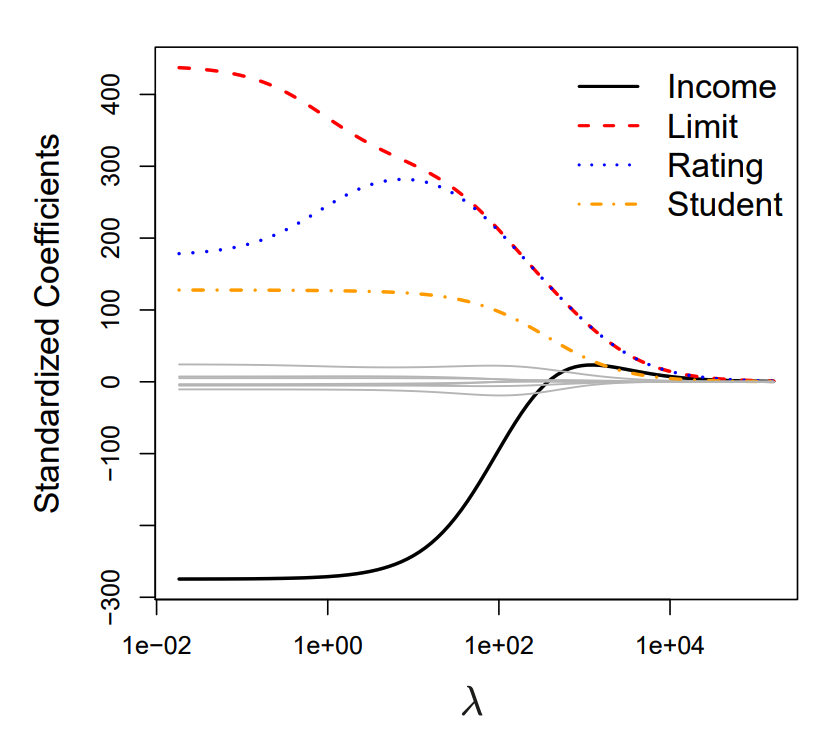
\includegraphics[width=7cm]{data/ridge_coefs.png}
            };
        }
        \only<5-6>{
            \node[align=center] at (2.675, 0) {
                $\hat{y}= \alert<6>{\beta_0} + \beta_1x_1 + \beta_2x_2$\\[0.25cm]
                $\ell=\sum\limits_{i=0}^n \left( y_i - \hat{y}_i \right)^2+\alert<6>{\lambda}\sum\limits_{j=0}^p \beta_j^2$\\[0.25cm]
            };
        }
        \only<7-8,11,17-25>{
            \node[align=center] at (2.675, 0) {
                $\hat{y}= \beta_1x_1 + \beta_2x_2$\\[0.25cm]
                $\ell=\alert<11-19>{\sum\limits_{i=0}^n \left( y_i - \hat{y}_i \right)^2}+\alert<20-23>{\sum\limits_{j=0}^p \beta_j^2}$\\[0.25cm]
            };
        }
        \only<8, 11-13>{
            \node[] at (-2.657, 0) {
                \ridgeintuition{1}
            };
        }
        \only<9>{
            \node[] at (-2.657, 0) {
                \ridgeintuition{2}
            };
            \node[align=center] at (2.675, 0) {
                $\hat{y}= \alert<9>{1}x_1 + \alert<9>{0}x_2$\\[0.25cm]
                $\ell=\sum\limits_{i=0}^n \left( y_i - \hat{y}_i \right)^2+\sum\limits_{j=0}^p \beta_j^2$\\[0.25cm]
            };
        }
        \only<10>{
            \node[] at (-2.657, 0) {
                \ridgeintuition{3}
            };
            \node[align=center] at (2.675, 0) {
                $\hat{y}= \alert<10>{1.5}x_1 + \alert<10>{1.5}x_2$\\[0.25cm]
                $\ell=\sum\limits_{i=0}^n \left( y_i - \hat{y}_i \right)^2+\sum\limits_{j=0}^p \beta_j^2$\\[0.25cm]
            };
        }
        \only<12>{
            \node[] at (2.675, 0.37) {
                \mseintuitionunivariate
            };
        }
        \only<13>{
            \node[] at (2.675, 0.37) {
                \mseintuitionbivariate{0}
            };
        }
        \only<14>{
            \node[] at (2.675, 0.37) {
                \mseintuitionbivariate{1}
            };
            \node[] at (-2.657, 0) {
                \ridgeintuition{4}
            };
        }
        \only<15>{
            \node[] at (2.675, 0.37) {
                \mseintuitionbivariate{2}
            };
            \node[] at (-2.657, 0) {
                \ridgeintuition{5}
            };
        }
        \only<16>{
            \node[] at (2.675, 0.37) {
                \mseintuitionbivariate{3}
            };
            \node[] at (-2.657, 0) {
                \ridgeintuition{6}
            };
        }
        \only<17>{
            \node[] at (-2.657, 0) {
                \ridgeintuition{7}
            };
        }
        \only<18>{
            \node[] at (-2.657, 0) {
                \ridgeintuition{8}
            };
        }
        \only<19-20>{
            \node[] at (-2.657, 0) {
                \ridgeintuition{9}
            };
        }
        \only<21>{
            \node[] at (-2.657, 0) {
                \ridgeintuition{10}
            };
        }
        \only<22>{
            \node[] at (-2.657, 0) {
                \ridgeintuition{11}
            };
        }
        \only<23>{
            \node[] at (-2.657, 0) {
                \ridgeintuition{12}
            };
        }
        \only<24>{
            \node[] at (-2.657, 0) {
                \ridgeintuition{13}
            };
        }
        \only<25>{
            \node[] at (-2.657, 0) {
                \ridgeintuition{14}
            };
        }

    \end{tikzpicture}
\end{frame}

\newsavebox{\predictorscales}
\sbox{\predictorscales}{
    \begin{tikzpicture}
        \begin{axis}[
            width=6cm,
            height=6cm,
            xlabel=Acceleration,
            ylabel=Weight
        ]
            \addplot[only marks, blue!50, opacity=0.5] table [col sep=comma, x=acceleration, y=weight] {data/Auto.csv};
        \end{axis}
    \end{tikzpicture}
}

\begin{frame}{Shrinkage: Feature standardization}
    \begin{tikzpicture}
        \node[] at (-5.4, -4) {};
        \node[] at (5.4, 3) {};

        \only<1-2>{
            \node[align=center] at (0, 0) {
                $y \sim \beta_0 + \beta_1x_1 + \beta_2x_2$\\
                $x_1 \in [0, 1], x_2 \in [0, 1000]$
            };
        }
        \only<2>{
            \node[rotate=270] at (0, -0.8) {
                $\Rightarrow$
            };
            \node[align=center] at (0, -1.2) {
                $\beta_1 \approx 1000*\beta_2$
            };
        }

        \only<3>{
            \node[] at (-0.5, -0.5) {
                \usebox{\predictorscales}
            };
        }
        \only<4-6>{
            \node[] at (0, 3) {\underline{\textbf{z-score standardization}}};

            \only<5-6>{
                \node[] at (0, 2.3) {
                    $\mathbf{x} = \frac{\mathbf{x} - \mu_x}{\sigma_x}$
                };
            }
            \only<6>{
                \PythonInputNode{1}{(-4.5, 1.5)}{pythonnode}{0.95\textwidth}{7}{
for col in predictors:^^J
{ }{ }{ }{ }print(f'\{col\}: \{np.mean(df[col]):.2f\} (\{np.std(df[col]):.2f\})')^^J
^^J
\# z-score standardization^^J
for col in predictors:^^J
{ }{ }{ }{ }df[col] = (df[col] - np.mean(df[col])) / np.std(df[col])^^J
^^J
for col in predictors:^^J
{ }{ }{ }{ }print(f'\{col\} after: \{np.mean(df[col]):.2f\} (\{np.std(df[col]):.2f\})')^^J
                }
                \PythonOutputNode{1}{(-4.39, -1.2)}{output}{0.882\textwidth}{7}{
cylinders: 5.47 (1.70)^^J
displacement: 194.41 (104.51)^^J
horsepower: 104.47 (38.44)^^J
cylinders after: -0.00 (1.00)^^J
displacement after: -0.00 (1.00)^^J
horsepower after: -0.00 (1.00)^^J
                }
            }
        }
    \end{tikzpicture}
\end{frame}

\begin{frame}{Shrinkage: Ridge regression}
    \begin{tikzpicture}
        \node[] at (-5.25, -3) {};
        \node[] at (5.25, 3) {};

        \node[inner sep=0pt] (loss) at (0, 0) {
            $loss_{ridge} = \sum\limits_{i=0}^n \left( y_i - \sum\limits_{j=0}^p \beta_j x_{ij} \right)^2 + \lambda \sum\limits_{j=0}^p$$\beta_j^2$
        };

        \node[font=\scriptsize] at (0, -1.5) {
            \url{http://localhost:8888/notebooks/notebooks/Live\%20coding.ipynb}
        };

    \end{tikzpicture}
\end{frame}

\newcommand{\lassointuition}[1]{
    \begin{tikzpicture}
        \begin{axis}[
            xmin=-2,
            xmax=5,
            ymin=-2,
            ymax=5,
            axis lines=middle,
            height=7cm,
            width=7cm,
            xtick={-2, -1, 0, 1, 2, 3, 4},
            ytick={-2, -1, 0, 1, 2, 3, 4},
            ticklabel style={font=\footnotesize},
        ]
            \node[] at (axis cs: -0.8, 2.5) {
                \footnotesize{$\beta_2$}
            };
            \node[] at (axis cs: 2.6, -0.8) {
                \footnotesize{$\beta_1$}
            };

            \ifnum#1=1
                \node[cross out, draw=black, thick, inner sep=0pt, minimum size=3pt, orange] at (axis cs: 1.5, 3.22) {};
                \draw[rotate around={20:(axis cs: 1.5, 3.22)}, orange] (axis cs: 1.5, 3.22, 2.7) ellipse (1cm and 0.5cm);
                \draw[rotate around={20:(axis cs: 1.5, 3.22)}, orange] (axis cs: 1.5, 3.22, 2.7) ellipse (1.414*1cm and 1.414*0.5cm);
                \draw[rotate around={20:(axis cs: 1.5, 3.22)}, orange] (axis cs: 1.5, 3.22) ellipse (1.732*1cm and 1.732*0.5cm);
            \fi
            \ifnum#1>1
                \node[cross out, draw=black, thick, inner sep=0pt, minimum size=3pt] at (axis cs: 1.55, 3.22) {};
                \draw[rotate around={20:(axis cs: 1.5, 3.22)}] (axis cs: 1.5, 3.22, 2.7) ellipse (1cm and 0.5cm);
                \draw[rotate around={20:(axis cs: 1.5, 3.22)}] (axis cs: 1.5, 3.22, 2.7) ellipse (1.414*1cm and 1.414*0.5cm);
                \draw[rotate around={20:(axis cs: 1.5, 3.22)}] (axis cs: 1.5, 3.22) ellipse (1.732*1cm and 1.732*0.5cm);
            \fi

            \ifnum#1<8
                \ifnum#1>2
                    \node[cross out, draw=black, thick, inner sep=0pt, minimum size=3pt, orange] at (axis cs: 0, 0) {};
                \fi
                \ifnum#1=4
                    \node[circle, inner sep=1pt, draw=orange, fill=orange] at (axis cs: 1, 0) {};
                    \node[circle, inner sep=1pt, draw=orange, fill=orange] at (axis cs: 0, 1) {};
                    \node[circle, inner sep=1pt, draw=orange, fill=orange] at (axis cs: -1, 0) {};
                    \node[circle, inner sep=1pt, draw=orange, fill=orange] at (axis cs: 0, -1) {};
                \fi
                \ifnum#1=5
                    \node[circle, inner sep=1pt, draw=orange, fill=orange] at (axis cs: 1, 0) {};
                    \node[circle, inner sep=1pt, draw=orange, fill=orange] at (axis cs: 0, 1) {};
                    \node[circle, inner sep=1pt, draw=orange, fill=orange] at (axis cs: -1, 0) {};
                    \node[circle, inner sep=1pt, draw=orange, fill=orange] at (axis cs: 0, -1) {};

                    \node[circle, inner sep=1pt, draw=orange, fill=orange] at (axis cs: 0.5, 0.5) {};
                    \node[circle, inner sep=1pt, draw=orange, fill=orange] at (axis cs: 0.5, -0.5) {};
                    \node[circle, inner sep=1pt, draw=orange, fill=orange] at (axis cs: -0.5, 0.5) {};
                    \node[circle, inner sep=1pt, draw=orange, fill=orange] at (axis cs: -0.5, -0.5) {};
                \fi
                \ifnum#1>5
                    \draw[orange] (axis cs: 1, 0) -- (axis cs: 0, 1) -- (axis cs: -1, 0) -- (axis cs: 0, -1) -- cycle;
                \fi
                \ifnum#1>6
                    \draw[orange] (axis cs: 2, 0) -- (axis cs: 0, 2) -- (axis cs: -2, 0) -- (axis cs: 0, -2) -- cycle;
                \fi
            \fi

            \ifnum#1=8
                \node[cross out, draw=black, thick, inner sep=0pt, minimum size=3pt] at (axis cs: 0, 0) {};
                \draw[] (axis cs: 1, 0) -- (axis cs: 0, 1) -- (axis cs: -1, 0) -- (axis cs: 0, -1) -- cycle;
                \draw[] (axis cs: 2, 0) -- (axis cs: 0, 2) -- (axis cs: -2, 0) -- (axis cs: 0, -2) -- cycle;
                \node[cross out, draw=black, thick, inner sep=0pt, minimum size=3pt, orange] at (axis cs: 0, 2) {};
            \fi

        \end{axis}
    \end{tikzpicture}
}

\begin{frame}{Shrinkage: LASSO}
    \begin{tikzpicture}
        \node[] at (-5.25, -3.5) {};
        \node[] at (5.25, 3.5) {};

        \only<1-2>{
            \node[inner sep=0pt] (loss) at (0, 0) {
                $loss_{ridge} = \sum\limits_{i=0}^n \left( y_i - \sum\limits_{j=0}^p \beta_j x_{ij} \right)^2 + \lambda \sum\limits_{j=0}^p\alert<2>{\beta_j^2}$
            };

            \node[inner sep=0pt] (lassomse) at (0, -1.5) {
                $loss_{lasso}= \sum\limits_{i=0}^n \left( y_i - \sum\limits_{j=0}^p \beta_j x_{ij} \right)^2 + \lambda \sum\limits_{j=0}^p\alert<2>{|\beta_j|}$
            };
        }
        \only<3-5>{
            \node[fill=white, draw=black, label=Ridge] at (-2.5, 1.5) {
                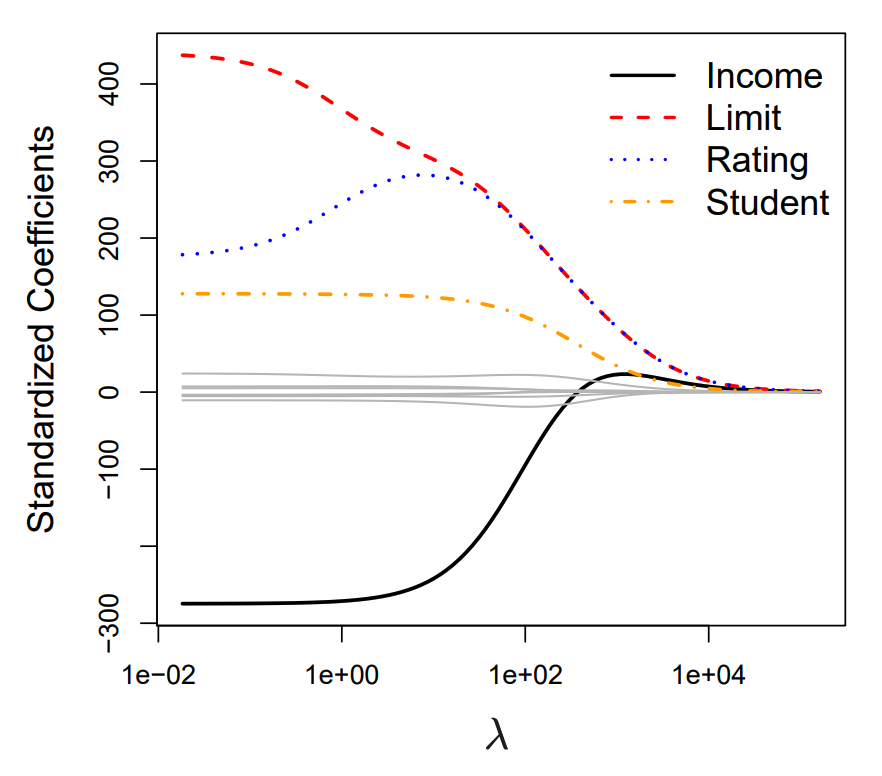
\includegraphics[width=3cm]{data/ridge.png}
            };
            \node[fill=white, draw=black, label=LASSO] at (2.5, 1.5) {
                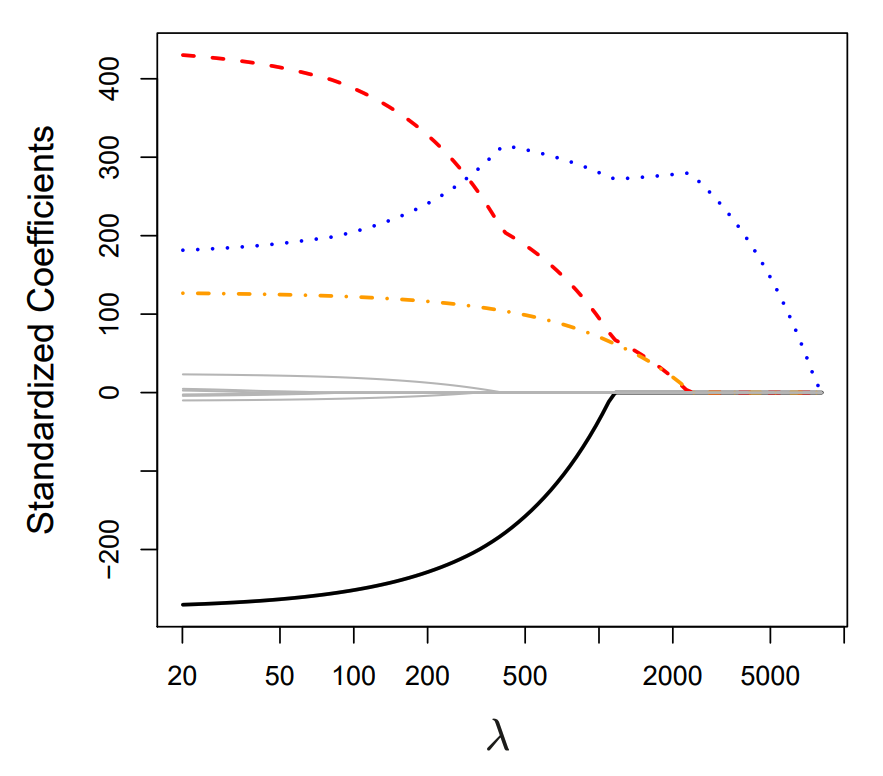
\includegraphics[width=3cm]{data/lasso.png}
            };
        }

        \only<4>{
            \node[] at (0, -2) {
                {\small
                    \begin{tabular}{|c|c|c|}
                        \hline
                        \textbf{Predictor}&\textbf{Ridge}&\textbf{LASSO}\\
                        \hline
                        Intercept&23.44&23.44\\
                        \hline
                        Weight&-5.59&-4.78\\
                        \hline
                        Year&2.75&2.00\\
                        \hline
                        Acceleration&0.19&0\\
                        \hline
                        Displacement&0.66&0\\
                        \hline
                    \end{tabular}
                }
            };
        }
        \only<6-13>{
            \node[align=center] at (2.675, 0) {
                $\hat{y}= \beta_1x_1 + \beta_2x_2$\\[0.25cm]
                $\ell=\alert<6>{\sum\limits_{i=0}^n \left( y_i - \hat{y}_i \right)^2}+\alert<7-12>{\sum\limits_{j=0}^p |\beta_j|}$\\[0.25cm]
            };
        }
        \only<6>{
            \node[] at (-2.675, 0) {
                \lassointuition{1}
            };
        }
        \only<7>{
            \node[] at (-2.675, 0) {
                \lassointuition{2}
            };
        }
        \only<8>{
            \node[] at (-2.675, 0) {
                \lassointuition{3}
            };
        }
        \only<9>{
            \node[] at (-2.675, 0) {
                \lassointuition{4}
            };
        }
        \only<10>{
            \node[] at (-2.675, 0) {
                \lassointuition{5}
            };
        }
        \only<11>{
            \node[] at (-2.675, 0) {
                \lassointuition{6}
            };
        }
        \only<12>{
            \node[] at (-2.675, 0) {
                \lassointuition{7}
            };
        }
        \only<13>{
            \node[] at (-2.675, 0) {
                \lassointuition{8}
            };
        }

        \only<14>{
            \node[] at (0, 1) {
                {\small
                    \begin{tabular}{|c|c|c|}
                        \hline
                        \textbf{Predictor}&\textbf{Ridge}&\textbf{LASSO}\\
                        \hline
                        Intercept&23.44&23.44\\
                        \hline
                        Weight&-5.59&-4.78\\
                        \hline
                        Year&2.75&2.00\\
                        \hline
                        Acceleration&0.19&0\\
                        \hline
                        Displacement&0.66&0\\
                        \hline
                    \end{tabular}
                }
            };
            \node[align=center] at (0, -2) {
                A coefficient of 0 does not mean the predictor has\\no association with the outcome! Why?
            };
        }
        \only<15>{
            \node[fill=white, draw=black] at (0, 0) {
                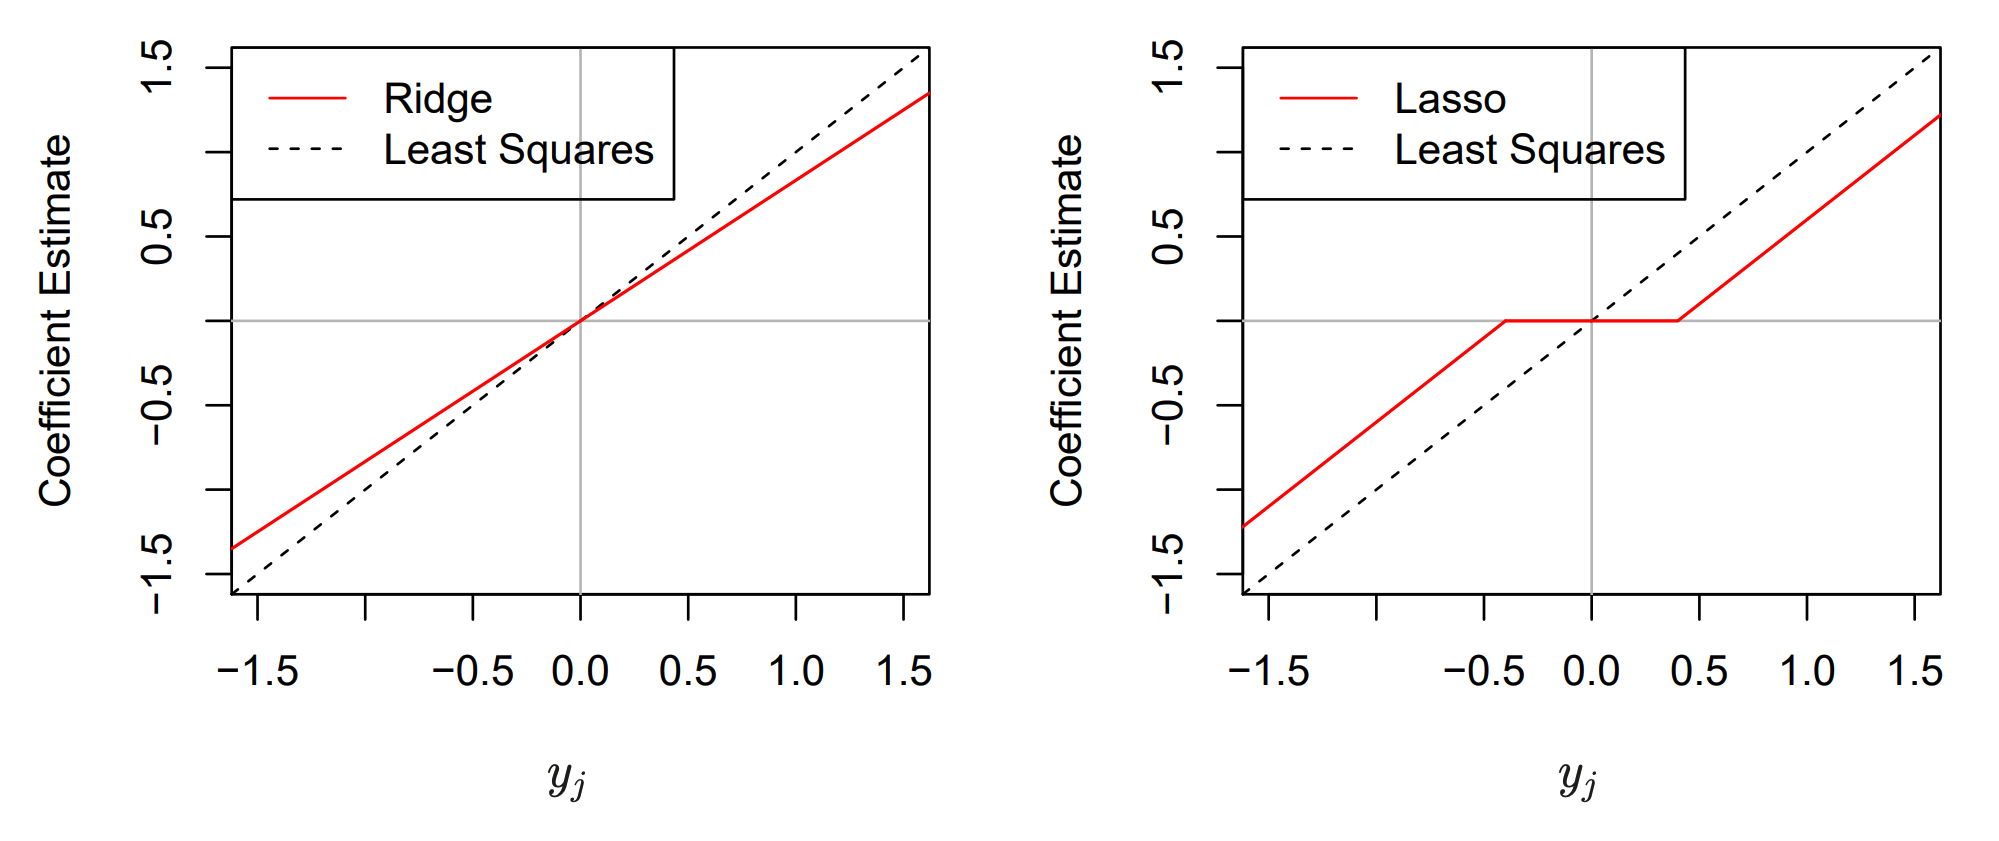
\includegraphics[width=10cm]{data/ridge_vs_lasso.png}
            };
        }
    \end{tikzpicture}
\end{frame}

\begin{frame}{Shrinkage: Summary}
    \centering
    \vfill
    \begin{tikzpicture}
        \node[] at (-5.25, 3.25) {};
        \node[] at (5.25, -3.25) {};

        \draw[black] (1, 3.25) -- (1, -3.5);

        \node[inner sep=0pt, font=\footnotesize, anchor=west] (mse) at (-5, 2.2) {
            $loss_{mse} = \sum\limits_{i=0}^n \left( y_i - \sum\limits_{j=0}^p \beta_j x_{ij} \right)^2$
        };
        \node[anchor=west, font=\footnotesize, align=flush left, text width=3.5cm] at ($ (mse.west) + (6.5, 0) $) {Fits the \textbf{best} model to the data.};

        \only<2-3>{
            \node[inner sep=0pt, font=\footnotesize, anchor=west] (ridgemse) at (-5, 0) {
                $loss_{ridge}= \sum\limits_{i=0}^n \left( y_i - \sum\limits_{j=0}^p \beta_j x_{ij} \right)^2 + \lambda \sum\limits_{j=0}^p \beta_j^2$
            };
            \node[anchor=west, font=\footnotesize, align=flush left, text width=3.5cm] at ($ (ridgemse.west) + (6.5, 0) $) {Fits the \textbf{best} model to the data while \textbf{shrinking} coefficients towards zero.};
        }

        \only<3>{
            \node[inner sep=0pt, font=\footnotesize, anchor=west] (lassomse) at (-5, -2.2) {
                $loss_{lasso} = \sum\limits_{i=0}^n \left( y_i - \sum\limits_{j=0}^p \beta_j x_{ij} \right)^2 + \lambda \sum\limits_{j=0}^p |\beta_j|$
            };

            \node[anchor=west, font=\footnotesize, align=flush left, text width=3.5cm] at ($ (lassomse.west) + (6.5, 0) $) {Fits the \textbf{best} model to the data while \textbf{shrinking} coefficients towards zero such that some variables are effectively \textbf{removed}.};
        }
    \end{tikzpicture}
    \vfill
\end{frame}
